\section{Exercises}

\begin{enumerate}
\item \emph{Nash Bargaining}

Consider a single access link and suppose that its bandwidth capacity $C$ is shared by $n$ users. Let $x_i$ denote the amount of bandwidth received by each user $i = 1,2,\ldots,n$, and suppose for simplicity that each user receives utility $x_i$ from $x_i$ amount of bandwidth. Suppose that the ISP allocates bandwidth to users so as to maximize
\begin{equation}
\prod_{i = 1}^n x_i\quad{\rm s.t.}\;\sum_{i = 1}^n x_i \leq C.
\end{equation}
Show that the resulting allocation $\left\{x_i^\ast\right\}$ satisfies the four Nash bargaining axioms presented in Section \ref{sec:gametheory}.

\item \emph{Time-of-Day Smart Grid Pricing}

Taken from M. Chiang, \emph{Networked Life: 20 Questions and Answers}, Cambridge University Press, 2012.
\\ \\
Smart grid electricity providers often set time-dependent prices for energy usage.  This problem considers a simplified example with two periods, the day-time and the night-time.  The provider can set different prices for the two periods, and wishes to shift some night usage to the day.  The energy provider always offers the full price during the night, and offers a reward of \$$p$/kWh during the day.

Suppose that with uniform (not time-dependent) prices, customers vacuum at night, using 0.2 kWh, and also watch TV, using 0.5 kWh, and do laundry, using 2 kWh.  During the day, customers use 1 kWh.  The probability of users shifting vacuum usage from the night to the day is
\begin{equation}
1 - \exp\left(-\frac{p}{p_V}\right),
\end{equation}
where $p_V = 2$, and the probability of shifting laundry to the daytime is
\begin{equation}
1 - \exp\left(-\frac{p}{p_L}\right),
\end{equation}
where $p_L = 3$.  Users never shift their TV watching from the night to the day.

Suppose that the provider has a capacity of 2 kWh during the night and 1.5 kWh during the day.  The marginal cost of exceeding this capacity is \$1/kWh.  Assume that energy costs nothing to produce until the capacity is exceeded.

\begin{enumerate}
\item
Compute the expected amount of vacuum and laundry energy usage (in kWh) that is shifted from the night to the day, as a function of $p$.
\item
Find (to the nearest cent) the reward $p$ which maximizes the energy provider's profit.
\item
Suppose that if vacuum or laundry usage is shifted from the night to the day, it is shifted by 12 hours.  Compute the expected time shifted of vacuum and laundry using $p = p^\ast$, the optimal reward found above.
\end{enumerate}

\item \emph{Paris Metro Pricing}

Taken from M. Chiang, \emph{Networked Life: 20 Questions and Answers}, Cambridge University Press, 2012.
\\ \\
Consider a metro system where two kinds of services are provided: service class $1$ and service class $2$. Let $p_1$, $p_2$ be the one-off fees charged per user when accessing service classes 1 and 2 respectively. Suppose each user is characterized by a valuation parameter $\theta\in [0,1]$ such that its utility of using service class $i$ is
$$U_{\theta}(i)=(V-\theta K(Q_i,C_i))-p_{i},$$
where $V$ is the maximum utility of accessing the service, $K(Q_i,C_i)$ measures the amount of congestion of service class $i$, given $Q_i\geq 0$ as the proportion of users accessing service class $i$ (with $\sum_i Q_i=1$), and $C_i\geq0$ is the proportion of capacity allocated to service class $i$ (with $\sum_i C_i=1$).

At the equilibrium, i.e., no user switches from his selection, $U_{\theta}(i)$ is merely a linear function of $\theta$. Suppose the equilibrium is illustrated as in Figure \ref{fig:equilibrium}.\\

\begin{figure}
\centering
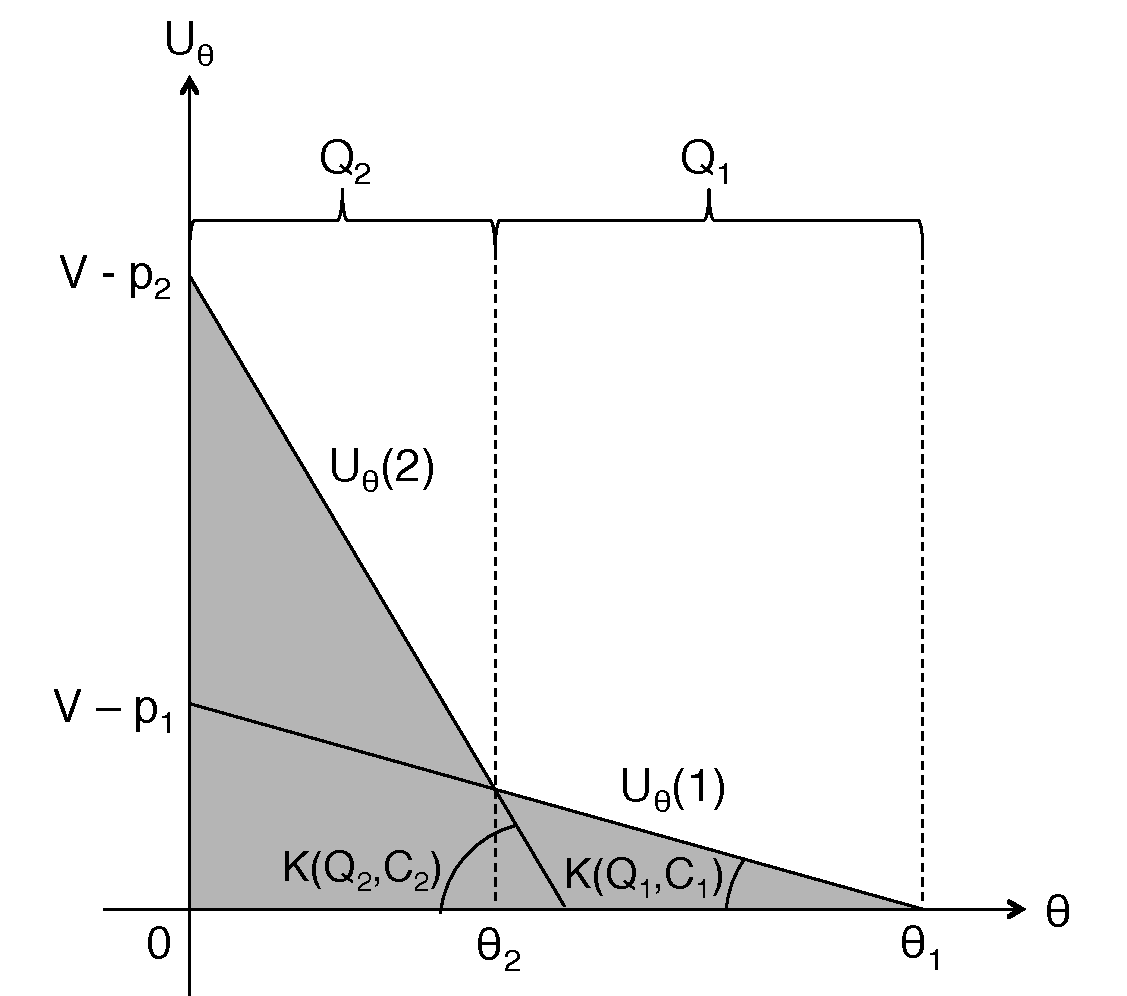
\includegraphics[width=8cm]{Figures/Equilibrium.pdf} 
\caption{\label{fig:equilibrium}Illustration of equilibrium in PMP.}
\end{figure}

Let $\theta_1$ be the $\theta$ of the user who is indifferent to joining the first service class or opting out of all the services, let $\theta_2$ be that of the user who is indifferent to joining the first service class or the second service class, and let $F(\theta)$ be the cumulative distribution function of $\theta$.
\begin{enumerate}
\item
Show that
\begin{subequations}
\begin{align*}
Q_1=&F(\theta_1)-F(\theta_2),\\
Q_2=&F(\theta_2),\\
V-p_1=&\theta_1 K(Q_1,C_1),\\
p_1-p_2=&\theta_2 (K(Q_2,C_2)-K(Q_1,C_1)).\\
\end{align*}
\end{subequations}

\item
Assume that $\theta$ is uniformly distributed, i.e., $F(\theta)=\theta$, and that the congestion function is defined as
$$K(Q,C)=\frac{Q}{C}.$$
Solve for $\theta_1$ and $\theta_2$ as functions of $V$, $p_1$, and $p_2$. 
\end{enumerate}

(Hint: Try $\frac{p_1-p_2}{V-p_1}$.)\\
 
(For details, see C. K. Chau, Q. Wang, and D. M. Chiu, ``On the Viability of Paris Metro Pricing for Communication and Service Networks," \emph{Proc. IEEE INFOCOM}, 2010.)\\

\item \emph{Two-Sided Pricing}

Taken from M. Chiang, \emph{Networked Life: 20 Questions and Answers}, Cambridge University Press, 2012.
\\ \\
Suppose an ISP charges a content provider (CP) the usage price $h_{CP}$ and flat price $g_{CP}$ and charges an end user (EU) the usage price $h_{EU}$ and flat price $g_{EU}$. For simplicity, we assume zero flat prices $\left(g_{CP}=g_{EU}=0\right)$. Let $\mu$ be the unit cost of provisioning capacity. The demand functions of the CP and EU, denoted as $D_{CP}$ and $D_{EU}$ respectively, are given as follows:\\
\begin{subequations}
\begin{align*}
D_{EU}(h_{EU})=&\left\{
\begin{array}{ll}
x_{EU,max}(1-\frac{h_{EU}}{h_{EU,max}})&\mbox{, if } 0\leq h_{EU}\leq h_{EU,max}\\
0,&\mbox{, if } h_{EU}>h_{EU,max}
\end{array}\right.\\
D_{CP}(h_{CP})=&\left\{
\begin{array}{ll}
x_{CP,max}(1-\frac{h_{CP}}{h_{CP,max}})&\mbox{, if } 0\leq h_{CP}\leq h_{CP,max}\\
0,&\mbox{, if } h_{CP}>h_{CP,max}.
\end{array}\right.\\
\end{align*}
\end{subequations}
The parameters are specified as follows:
\begin{subequations}
\begin{align*}
h_{CP,max}&=2.0\mu,\\
h_{EU,max}&=1.5\mu,\\
x_{CP,max}&=1.0,\\
x_{EU,max}&=2.0.\\
\end{align*}
\end{subequations}
The ISP maximizes its profit by solving the following maximization problem
\begin{equation}
\begin{array}{ll}
\mbox{maximize}	&(h_{CP}+h_{EU}-\mu)x\\
\mbox{subject to}	&x\leq \mbox{min}\{D_{CP}(h_{CP}),D_{EU}(h_{EU})\}\\
\mbox{variables} 	&x\geq 0, h_{CP}\geq 0, h_{EU}\geq 0.
\end{array}
\end{equation}

Find the optimal $x^\star, h_{CP}^\star, h_{EU}^\star$.\\

\item \emph{Monitoring Mobile Data Usage}

Many commercial mobile applications have been developed to help users keep track of their mobile data usage. Some examples include 3GWatchdog Pro (Android), DataWiz (iOS and Android), MyDataManager (Android), and Onavo Count (Android and iOS).
\begin{enumerate}
\item
Visit two or three app websites and list their features (e.g., showing usage by application, forecasting future usage, alerts when you approach your monthly data quota). Are there any significant differences between the apps? Can you identify any consistent differences between iOS and Android apps?
\item
What visual elements are used in the app designs? For instance, do the apps use bars or pie charts to represent usage? How are these displays different on different apps?
\item
Based on your answers to the above questions, try to design your own app for tracking mobile data usage. What screens would you implement? What features would you offer?
\end{enumerate}
\end{enumerate}